\chapter{Multi-task learning}

So far we have considered \ac{AES} and \ac{NLI} as independent tasks and
performed experiments on both tasks separately. We will now try to train
models to predict both tasks simultaneously.


\section{Models}

We selected four models for the multi-task experiments, two convolutional and
two recurrent neural networks. They were chosen based on the macro \FI results
on the development set. The two \acp{CNN} chosen were the two \acp{CNN} that
had the highest macro \FI on the full set of labels in the development set,
and likewise for the two \acp{RNN}. The hyperparameters for the four models are
summarized in tables \ref{tab:cnn-parameters} and \ref{tab:rnn-parameters}.

\begin{table}
  \centering
  \begin{tabular}{lll}
    \toprule
    Hyperparameter & CNN1 & CNN2 \\
    \midrule
    Embedding size & \multicolumn{2}{c}{100} \\
    $L_2$ constraint & \multicolumn{2}{c}{3} \\
    Embedding init & Random & Pre-trained \\
    Input representation & Mixed UPOS & Tokens \\
    \bottomrule
  \end{tabular}
  \caption{Descriptions of the two CNN models}
  \label{tab:cnn-parameters}
\end{table}

\begin{table}
  \centering
  \begin{tabular}{lll}
    \toprule
    Hyperparameter & RNN1 & RNN2 \\
    \midrule
    Word embeddings & \multicolumn{2}{c}{Dynamic} \\
    Embedding size & \multicolumn{2}{c}{100} \\
    RNN cell & \multicolumn{2}{c}{GRU} \\
    Pooling method & \multicolumn{2}{c}{Attention} \\
    Bidirectional & \multicolumn{2}{c}{Yes} \\
    Embedding init & Random & Pre-trained \\
    Input representation & Tokens+UPOS & Tokens \\
    \bottomrule
  \end{tabular}
  \caption{Descriptions of the two RNN models}
  \label{tab:rnn-parameters}
\end{table}

We chose ten different auxiliary loss weights, and for each loss weight we
trained and evaluated each model five times with different random seeds. By
training more than one model with a given set of hyperparameters, we can get
an idea of the variance of results.


\section{Results}

Below we plot see the results of running some of
the most successful models from the previous chapter in a multi-task setting,
using the essay's L1 as the auxiliary label to predict. The $x$ value
is the weight given to the auxiliary loss during training. An auxiliary loss
weight of 0 is the same as single-task setup.

The reported metrics apply to the main task, CEFR prediction, only. It seems
that the auxiliary task is beneficial for all CNN models. All CNN models get
higher macro and micro \FI in the multi-task setup. Moreover, a higher weight
given to the auxiliary L1 prediction task seems to improve macro \FI
performance across the board. The effect of the auxiliary task weight seems
less clear on the micro \FI, but remember that in our setup, the micro \FI is
a side effect of the highest macro \FI seen during training.

\todo{new models}
\todo{graph effect of loss weight on metrics}

\begin{figure}
  \centering
  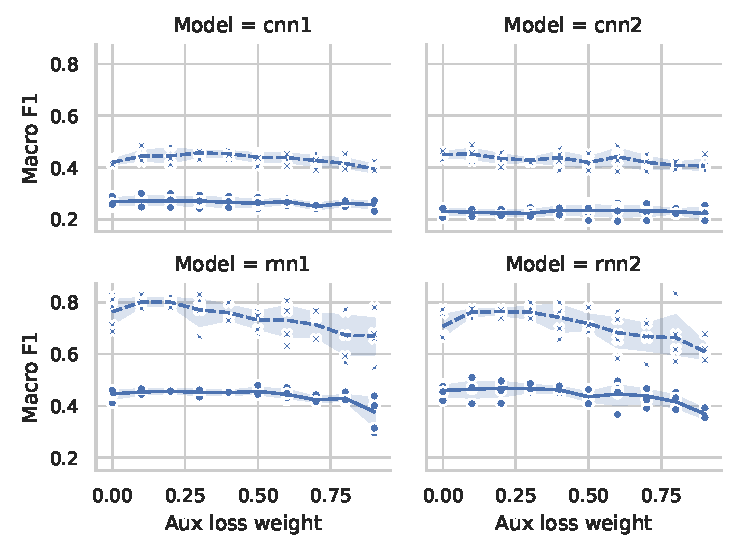
\includegraphics{lossweight}
  \caption[Performance of multi-task models]{
    Lines follow the mean of macro \FI scores. Shaded areas show 95\% confidence
    interval for mean. Results for the collapsed set of classes are plotted with
    cross symbols and dashed lines.
  }
  \label{fig:lossweight}
\end{figure}

The highest macro \FI scores on the full label set all come from the RNN2 model.
The five highest scores range between $0.486$ and $0.509$ and were achieved
using auxiliary loss weights in the range from $0.1$ to $0.6$.


\todo{do this}
Something with the confidence intervals


For the RNNs, the results are not quite as clear. The multi-task models were
not able to exceed the macro \FI scores of $0.354$ (all labels) and $0.624$
(collapsed labels), but this may be because the macro \FI metric is unstable
because of the `A2' class with one single example in the dev set. For the
same models, accuracy did increase in the multi-task setup.t

The model `RNN1 0.5' was the best performing multi-task model by several
metrics. In addition to macro \FI, it was the best in terms of RMSE
($0.888$), MAE ($0.610$), Pearson's correlation coefficient ($0.765$) and
Spearman's ranked correlation coefficient ($0.768$).


\begin{figure}
  % cnn-multi-26199963_11
  \begin{subfigure}{\linewidth}
    \centering
    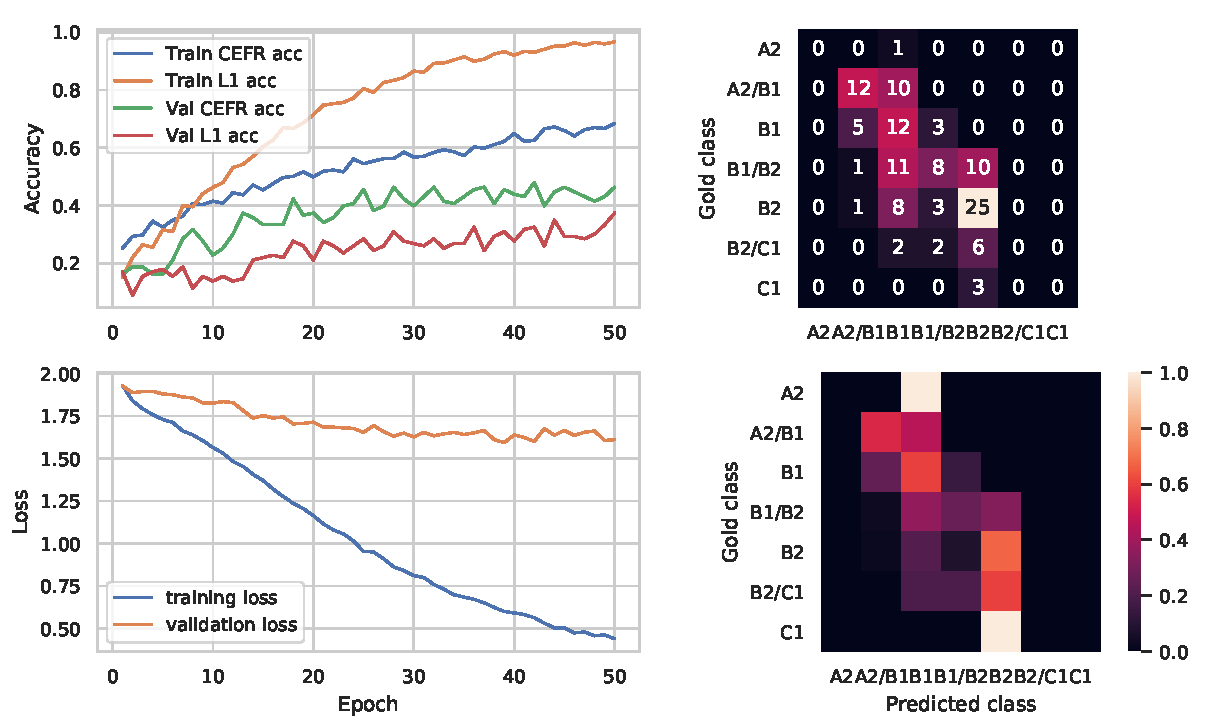
\includegraphics{cnn-multi-training}
    \caption{Training and validation loss and accuracy over 50 epochs of training.}
  \end{subfigure}
  \begin{subfigure}{\linewidth}
    \centering
    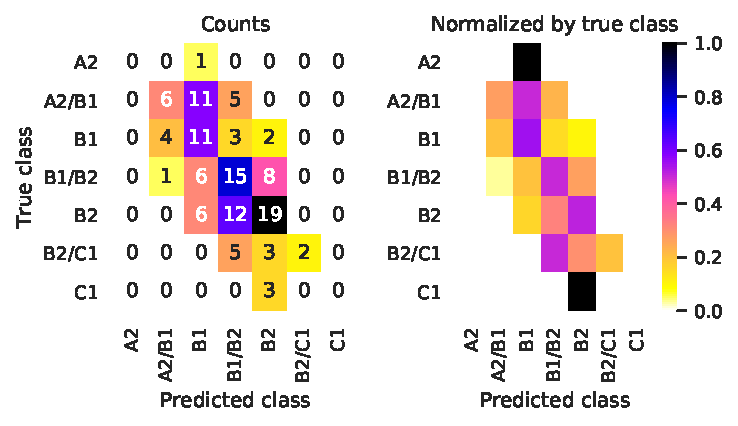
\includegraphics{cnn-multi-confusion}
    \caption{Confusion matrix on validation set, raw counts and normalized.}
  \end{subfigure}
  \caption{CNN2 0.75}
  \label{fig:cnn-multi-training}
\end{figure}

\begin{figure}
  % rnn-multi-26199963_15
  \begin{subfigure}{\linewidth}
    \centering
    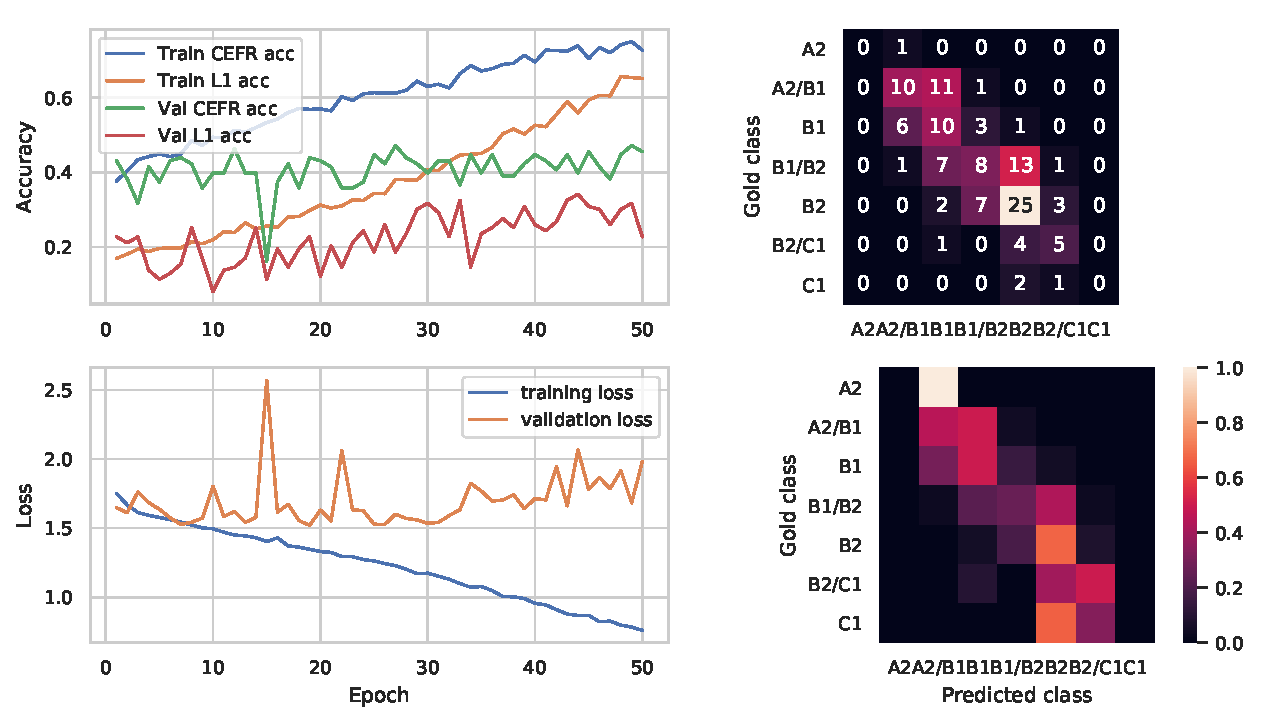
\includegraphics{rnn-multi-training}
    \caption{Training and validation loss and accuracy over 50 epochs of training.}
  \end{subfigure}
  \begin{subfigure}{\linewidth}
    \centering
    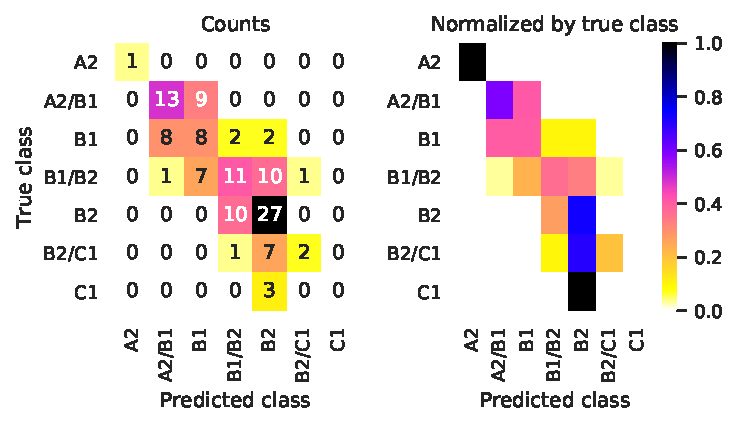
\includegraphics{rnn-multi-confusion}
    \caption{Confusion matrix on validation set, raw counts and normalized.}
  \end{subfigure}
  \caption{RNN1 0.5}
  \label{fig:rnn-multi-training}
\end{figure}


\section{Correlation of metrics}

\todo{More different metrics}

We have previously discussed different evaluation metrics. Since we now have
trained and evaluated a number of different models, it is possible to see whether
the metrics agree on the ranking of models.

Macro \FI and macro \ac{MAE} correlates only weakly, as seen in figure
\ref{fig:f1-vs-mae}, but they seem to agree on the highest ranking models:
The Pareto front consists of only two samples. The samples in the plot are
models that predict the full seven classes.

\begin{figure}
  \centering
  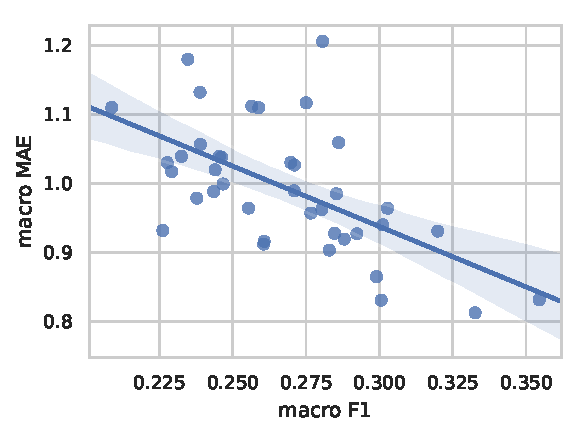
\includegraphics{f1-vs-mae}
  \caption[Macro \FI versus macro MAE]{
    Macro \FI versus macro MAE. Pearson's correlation coefficient = $-0.5945$,
    $p < 10^{-4}$. The shaded area covers a 95\% confidence interval for the
    line of regression.
  }
  \label{fig:f1-vs-mae}
\end{figure}
